\chapter{Molecular Dynamics (MD): force field development}


Very useful and accessible review papers I found browsing the net:
\begin{enumerate}
    \item Chodera, Noe, \textit{Markov state modeling of conformational dynamics} \url{doi:10.1016/j.sbi.2014.04.002}
    \item Hollingsworth, Dror, \textit{Molecular dynamics simulations for all}, \url{doi:10.1016/j.sbi.2014.04.002}.
\end{enumerate}

In the remaining of the chapter I report instead only the content of professor Fuxreiter lessons.
\section{Introduction (Lecture Thu, 9th April)}

So, what you had done largely until now is to describe biological systems, also protein systems, through data without looking at the very origin of this data. 
Today as I said we start something different. We want to use approaches where we are certain about the origins. We can do heavy approximations, but we will know our approximations, we will know about their effect. And we'll try to see how far we get through this approach. 

\paragraph{Areas of application}
So we will be busy with this kind of, let's say, approach all April, and in May we'll try to integrate the two. So basically when you try to understand how a chemical reaction takes place in a protein, in a large and complex entity, you cannot avoid using some kind of physical insights like describing not only the actual reaction like this movie, which by the way is a very interesting multiscale simulations that I might mention at the very end. So here obviously you need some quantum chemistry and then you move to the next. But at the end of the day, what you really need is not the movie itself, but understanding the free energy profile of the whole process and understanding how different parts of this very complex object contribute to this free energy pathway. 

If you want to do something else—and this is by the way, this is something that you need if someone has a disease mutation with some of their metabolic pathway—this is what you need to understand why that mutation affects the free energy pathway, why that mutation let's say prohibits the reaction going. Maybe it's because of the reaction itself directly, or maybe it's because of some regulatory features. 

But the other big area, if you want to understand some structural changes in proteins—in particular, we are very much interested in changes that are associated with advanced age. We had discussed many lectures ago the stability of beta-strands or beta-sheets which are associated with a number of diseases, neurological disorders that come with cognitive decline. So these are just examples of cases where you can also obviously use some kind of database thing, but to get a real insight, the deep insight, you cannot basically you cannot avoid using the approaches with clear physical origins. 


\begin{figure}[H]
    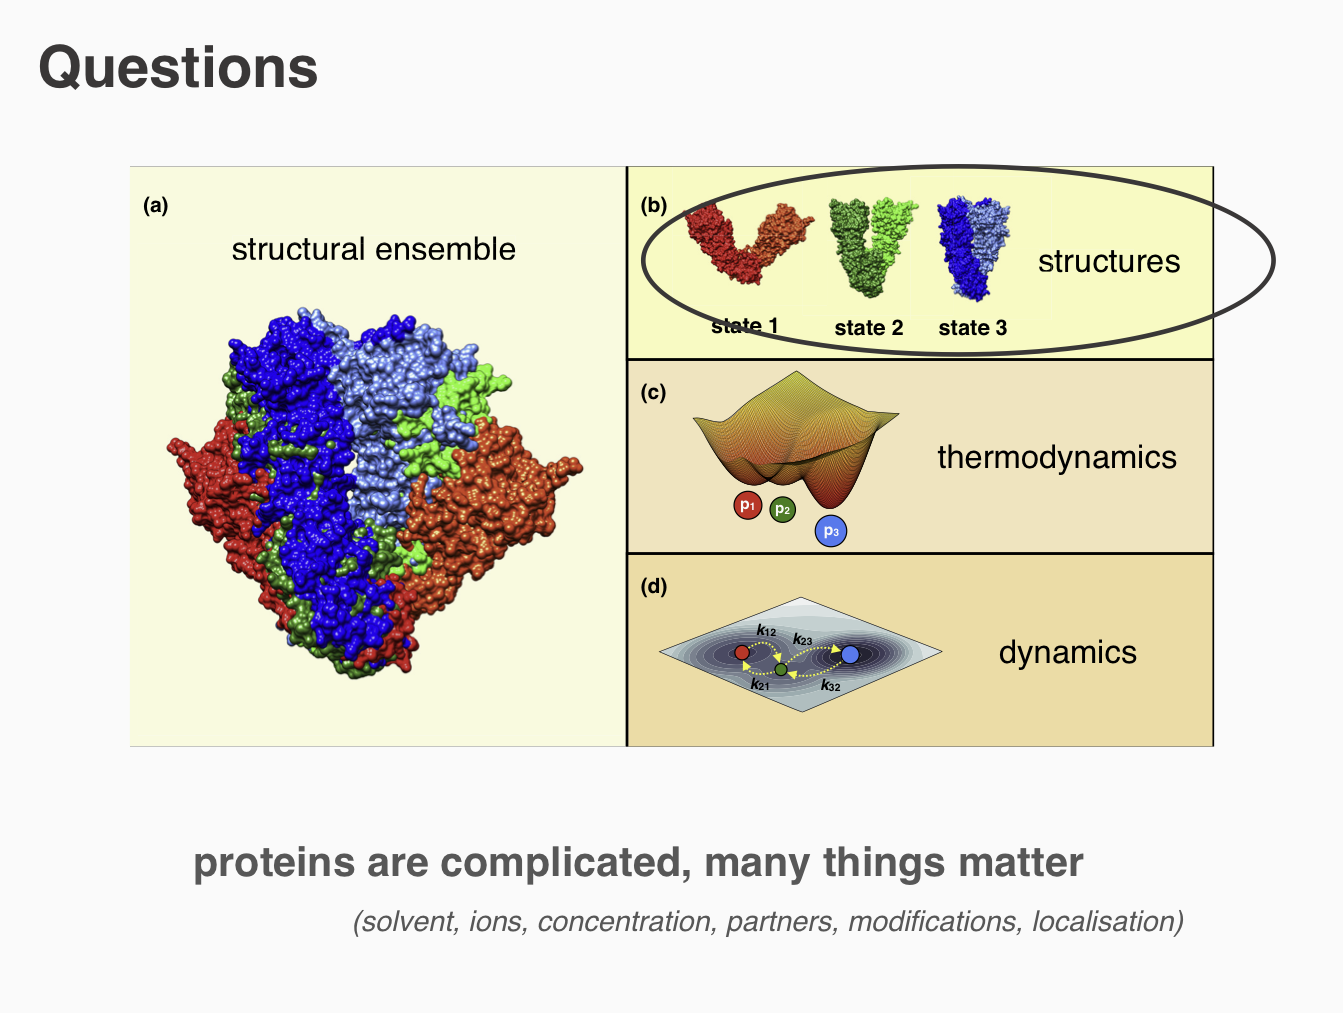
\includegraphics[width = \textwidth]{slides/simulations/questions.png}
\end{figure}

There are three main questions that you can ask for this kind of physics-based approaches. From the most easy to the most difficult:

\begin{enumerate}
    \item \textbf{Structure:} identifying the \textit{basins} in the potential energy surface (PES). In the canonical ensemble, the probability density of a microstate $\mathbf{x}$ is given by $p(\mathbf{x}) \propto e^{-\beta{U(\mathbf{x})}}$. So this is a minimization problem on a very high-dimensional function. Local minima are then clustered into a discrete set of basins, which correspond to the stable \textit{macrostates} of the biomolecule, or \textbf{conformers}.
    \item \textbf{Thermodynamics:} finding the \textit{relative occupancy} of these macrostates, or \textbf{conformer rations}. In the canonical ensemble, the probability of a macrostate depends not only on the energy $U$, but on the free energy $F= U-TS$: $P(U) \propto e^{-\beta(U - TS)}$. Equivalently, it is found by integrating the probability over the microstates. The entropic contribution ($-TS$) is linked to
           the \textit{width} of the basins: a wide basin implies there are a lot of microstates available to explore, so the probability of the associated macrostate will be higher.
    \item \textbf{Kinetics:} characterize pathways of conformational transition. This involves estimating quantities such as transition probabilities, rate constants, or mean first passage times. It typically requires identifying suitable \textit{reaction coordinates} or state decompositions and constructing reduced dynamical models (e.g., \textit{Markov state models}) to access long-timescale behavior beyond direct simulation.
\end{enumerate}

So these are distinct questions. Apart from this, you can ask many others, like for example the free energies of of a reaction. This would be free energy difference between a minimum and a saddle point.

\paragraph{You must choose the right \textit{scale} for the right question}

\begin{figure}[H]
    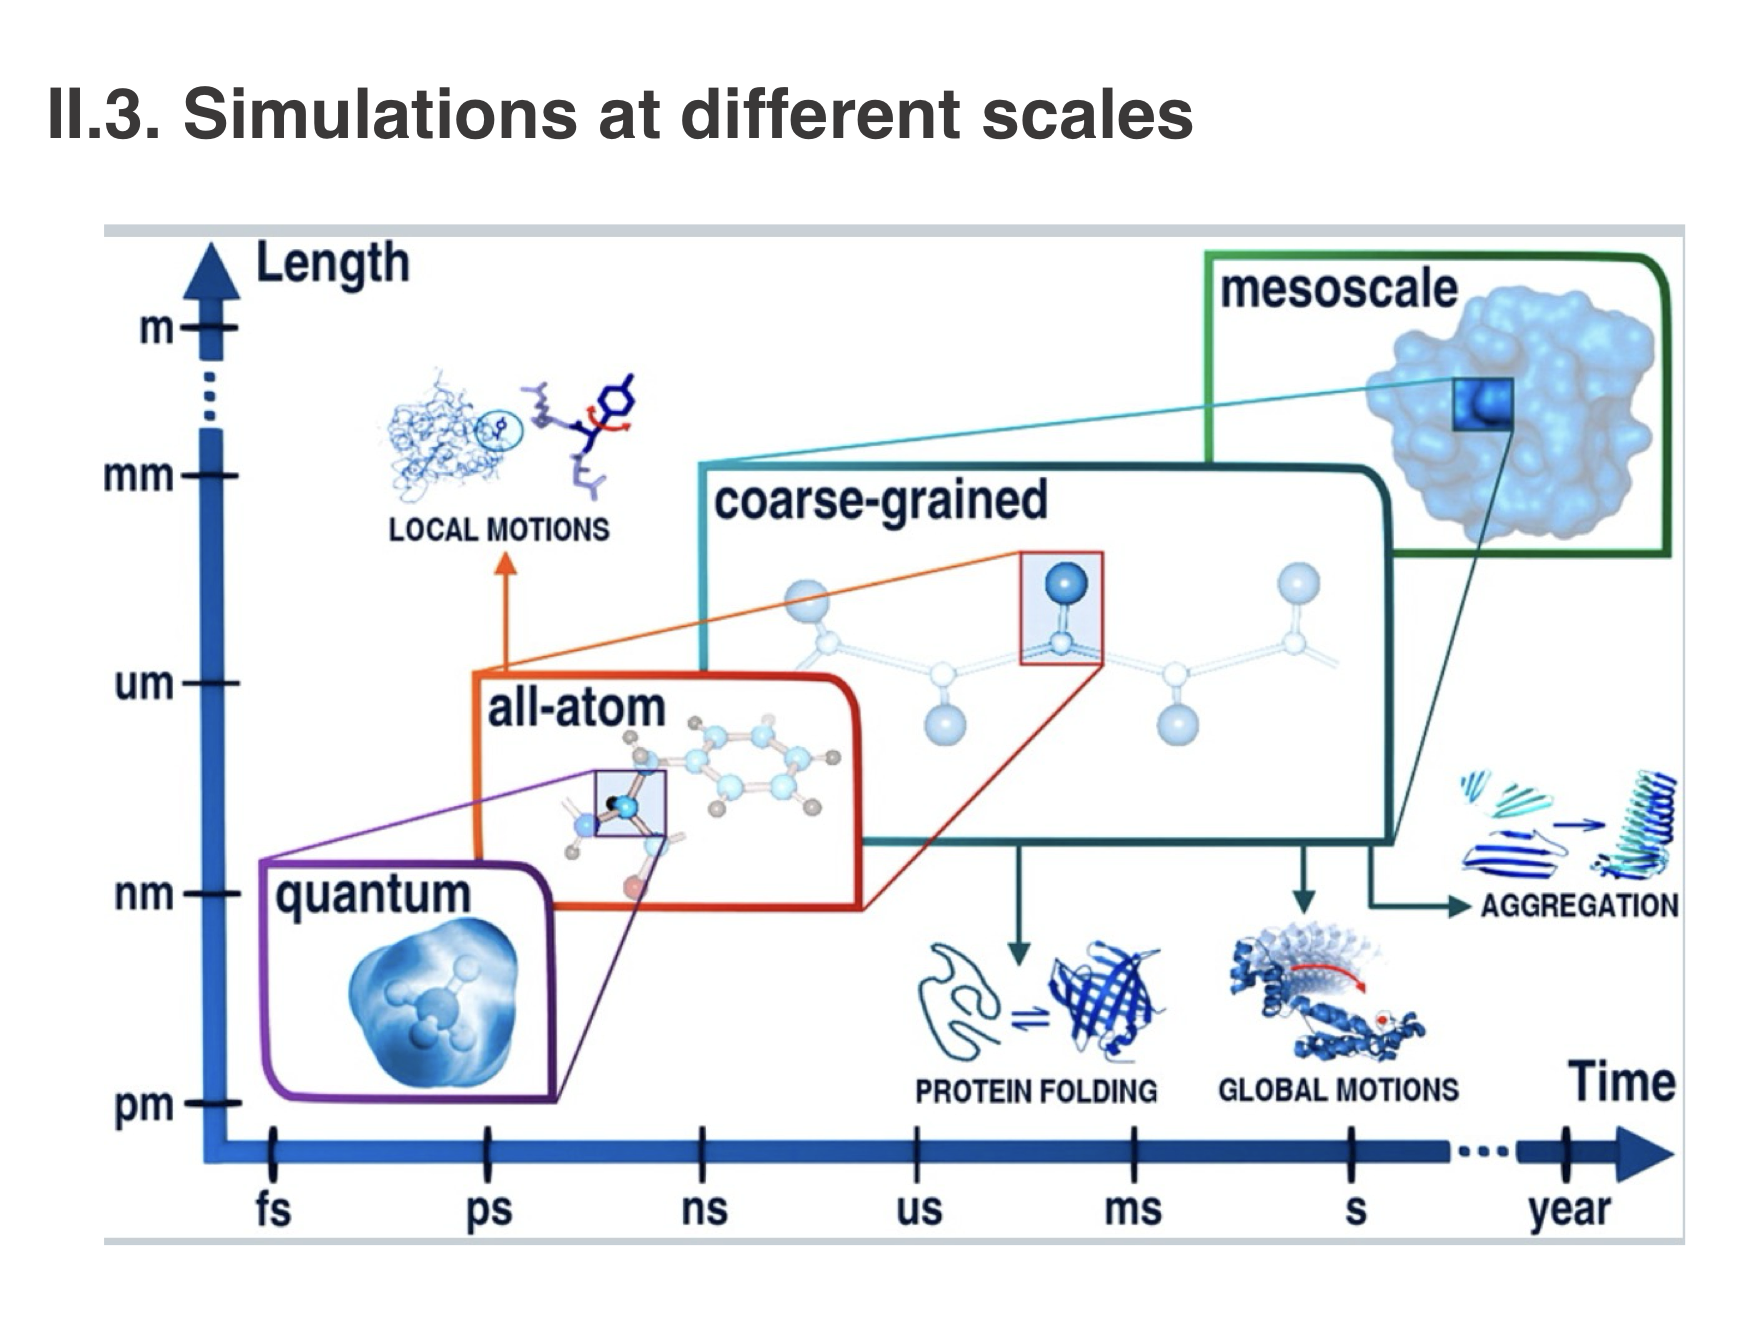
\includegraphics[width = \textwidth]{slides/simulations/different_scales.png}
\end{figure}

But just looking at this graph—which is a very simple intro graph, \textbf{force fields are growing like mushrooms} after the rain in the forest. So by the time you graduate there will be three new out-breaking force fields and so on. 

Whatever comes, \textbf{the first thing you need to map the new force field on this scale}, and you would need to relate—map—to the actual biological question that you want to study. The two must be comparable, the two the scales must overlap in order to start the right question for the right simulation. This is one of the key take-home messages of today and then we will elaborate. 


\paragraph{Simulations mostly use classical mechanics}


We are obliged in a way, if you want to answer questions which are on a longer timescale, which include many thousands of atoms, we may be obliged to to simplify.
So basically we want to move all classical. Okay? We want to use classic mechanical equations. We want to generate basically forces; the forces are generated based on the potential energy surface that we define. So we derive the forces from there. We will have starting positions, normally from experimental structures—nowadays sometimes from AlphaFold—and you assign velocities. Normally you assign velocities randomly, but we will discuss it also. 

But this is what is your goal, but to achieve this goal and to have the right and smooth surface to move and have the right, let's say, forces that the surface that you can compute the derivatives of, it's a bit challenging. 

So the very first thing you need to do is to make some approximations. And in—well, in general, in simulations you make a huge number of approximations. Okay? You cannot avoid that. That's fine. The main point is that you need to understand what you have done and you need to clearly write down for yourself: what is the impact of that simplification for your system? So what is the feature, what is the characteristic, that you are going to miss simply because you made that approximation? 

That's really crucial because \textbf{when we are modeling, we are mapping the real system into something that is obviously not real, but at the end of the day we would like to make predictions, we would like to map it back}. We can tell the biologist or pharmaceutical chemist: 'Make a mutation there, put a small molecule there, and your molecule will operate differently.' 

So the main approximations we make is basically as follows. We cannot solve the time-dependent Schrödinger equation for multiple nuclei and electrons. So because of that, because of that, we will be obliged basically to use the Born-Oppenheimer approximation and basically separate the nuclei motion from the electronic motion. Okay? So basically we make the total wave function as a product of the two. Okay? Both of them can be described in a fairly simple manner from the kinetic energy and from the electrostatic energy. The electro—in case of the electrons, the electrostatic energy in particular the one in between the electrons is very complicated—you need complicated methods like the Hartree-Fock method for example to deal with this or more advanced methods to correct MPI methods, DFT, whatever. So there are many ways. 

But anyway, the basic thing that you assume that whenever the nuclei moves, at that static position, you can compute the energies of the electrons for that particular configuration. And there is no basically there is no apart from the mere Coulombic attraction, there is no interference between the two motions. Again, this is a very strong approximation and there are methods to overcome it, but their sampling, so the time ranges that we can achieve with those is pretty short. Okay? 

So basically for the nuclei, obviously you can generate the similar Hamiltonian operator. And basically then what you want based on this: that you generate a potential energy surface, okay, which is a function of the nuclear coordinates. Okay? So basically you want to generate an energy where you will not solve the Schrödinger equation, okay? You approximate the Schrödinger equation; you approximate the Schrödinger equation just for the nuclear coordinate. Okay? You want to get something which approximates the electronic Schrödinger equation. 

Okay, but we will not see—I mean this was the last time you you had seen anything of quantum chemistry so far. You will forget about all the formalisms, okay? You will basically simplify to a multi-dimensional surface. Okay? 


So basically when you do the physics—physics-based approach, okay, you have two tasks: 

\begin{enumerate}
\item \textbf{Define this potential energy surface (PES)}. The derivatives would give you all the forces. This is the basis of everything: the quality of your simulation will depend on the quality of your PES. You need to understand that this is a crucial step.
\item  \textbf{Sample} The simulation itself: exploring the landscape. The sampling issue—exploring this, finding the minima, global minima, finding some transition point, saddle point, going from one minimum to another—this is all extremely challenging.
\end{enumerate}



\section{Force Field development: defining the PES.}
In the remaining of this lecture we talk extensively about thew common basis of force field development, so that you can understand
how to choose a force field that is appropriate for \textit{your} problem.

Approximations
\begin{enumerate}
    \item Born-Oppenheimer approximation ($\Phi _{mol} = \Phi_{nuc}\times \Phi_{el}, \quad E_{mol} = E_{nuc} + E_{el}$),
    \item energy is the sum of \textit{pairwise} interactions (?),
    \item separation of conformational energy into distinct terms (bond stretch, angle bend, torsion), modeled using simple mechanical functions,
    \item atoms are represented by hard spheres of radius $r$, with a \textit{point} electrical charge.
\end{enumerate}


\subsection{Atomic properties}

\paragraph{Atomic radius}

Assigning a radius to an atom is tricky, because as you all know, electron density decays smoothly and there exists no sharp boundary marking the end of an atom. So what we do is define an \textit{effective} radius derived from experiments. Typically, X-ray or electron diffraction, which give a typical interatomic distance in crystals.

But interatomic distance is not fixed. There are \textbf{Van Der Waals} forces. he force results from a transient shift in electron density. Specifically, the electron density may temporarily shift to be greater on one side of the nucleus. This shift generates a transient charge which a nearby atom can be attracted to or repelled by. The force is repulsive at very short distances, reaches zero at an equilibrium distance characteristic for each atom, or molecule, and becomes attractive for distances larger than the equilibrium distance. For individual atoms, the equilibrium distance is between 0.3 nm and 0.5 nm, depending on the atomic-specific diameter.
The Lennard-Jones potential is often used as an approximate model for the isotropic part of a total (repulsion plus attraction) van der Waals force as a function of distance.
\begin{figure}[H]
    \centering
    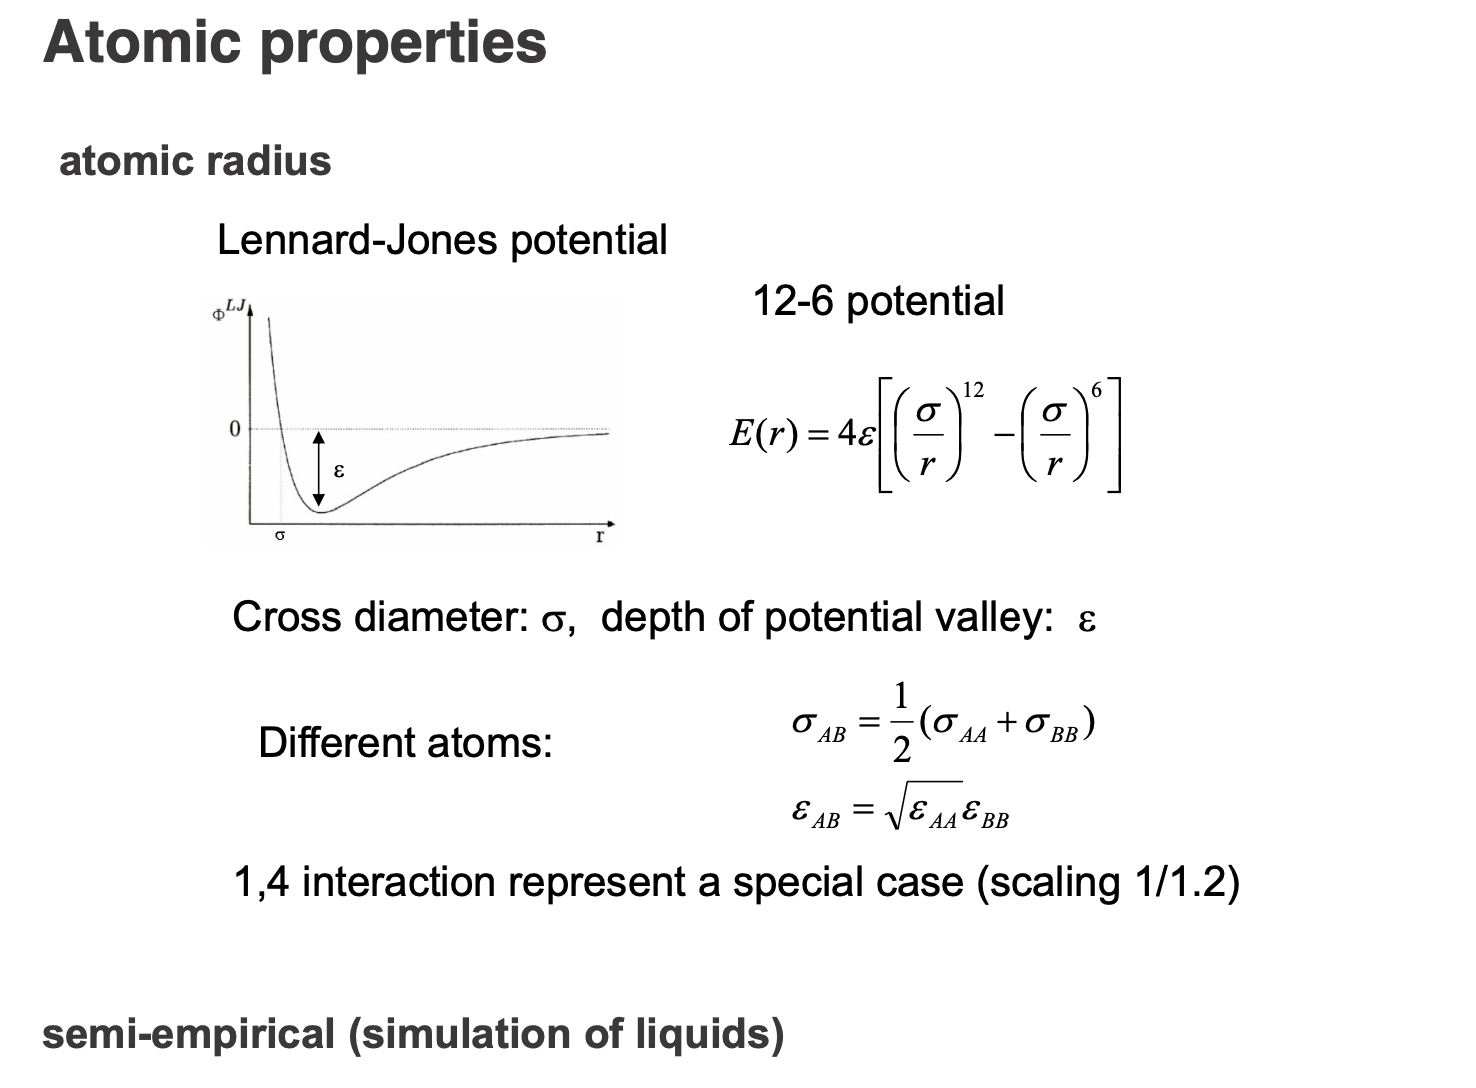
\includegraphics[width = 0.8\textwidth]{slides/simulations/lennarjones.png}
    \caption{The Lennard-Jones potential is a simple model that still manages to describe the essential features of interactions between simple atoms and molecules: two interacting particles repel each other at very close distances, attract each other at moderate distances, and eventually stop interacting at infinite distance, as shown in the figure. The Lennard-Jones potential is a pair potential, i.e. no three- or multi-body interactions are covered by the potential}
\end{figure}


You try to perform simulations with very simple potentials of this kind, and then you can try to parameterize the values. I mean, basically here you need to get the epsilon, you need to get the sigma, and also you need to refine the r. 
You can get good guesses (from experiments), but in fact at the end of the day you need to run the simulation to refine all these parameters (your simulation should reproduce experimental observables). Kind of trial and error. 



\paragraph{Atomic charge}


\begin{enumerate}
    \item \textbf{Atomic charges in a biomolecule are conformation-dependent}: First of all, the atomic charges—not only that these are not physical parameters, but highly dependent on the conformation of the molecule. So if if—in particular if you imagine a highly complex molecule, it can turn towards, let's say, you had a more positively charged atom, it can turn towards more negatively charged residues then the charges the charge may be reduced, okay, or can turn towards more positively charged—no, so anyway it depends highly on the conformation. 
    \item \textbf{We only consider first order Coloumb interactions:} and ignore all higher order interactions coming from the expansion of the Coloumb potential (dipole-dipole, dipole-quadrupole, etc)
    \item \textbf{Dielectric constant is highly inhomogeneous in a biomolecule:} Also the dielectric constant, which we take as a constant value normally, it's not at all constant. It's it's very inhomogeneous in proteins, as very difficult to guess actually. 
\end{enumerate}


\begin{figure}[H]
    \centering
    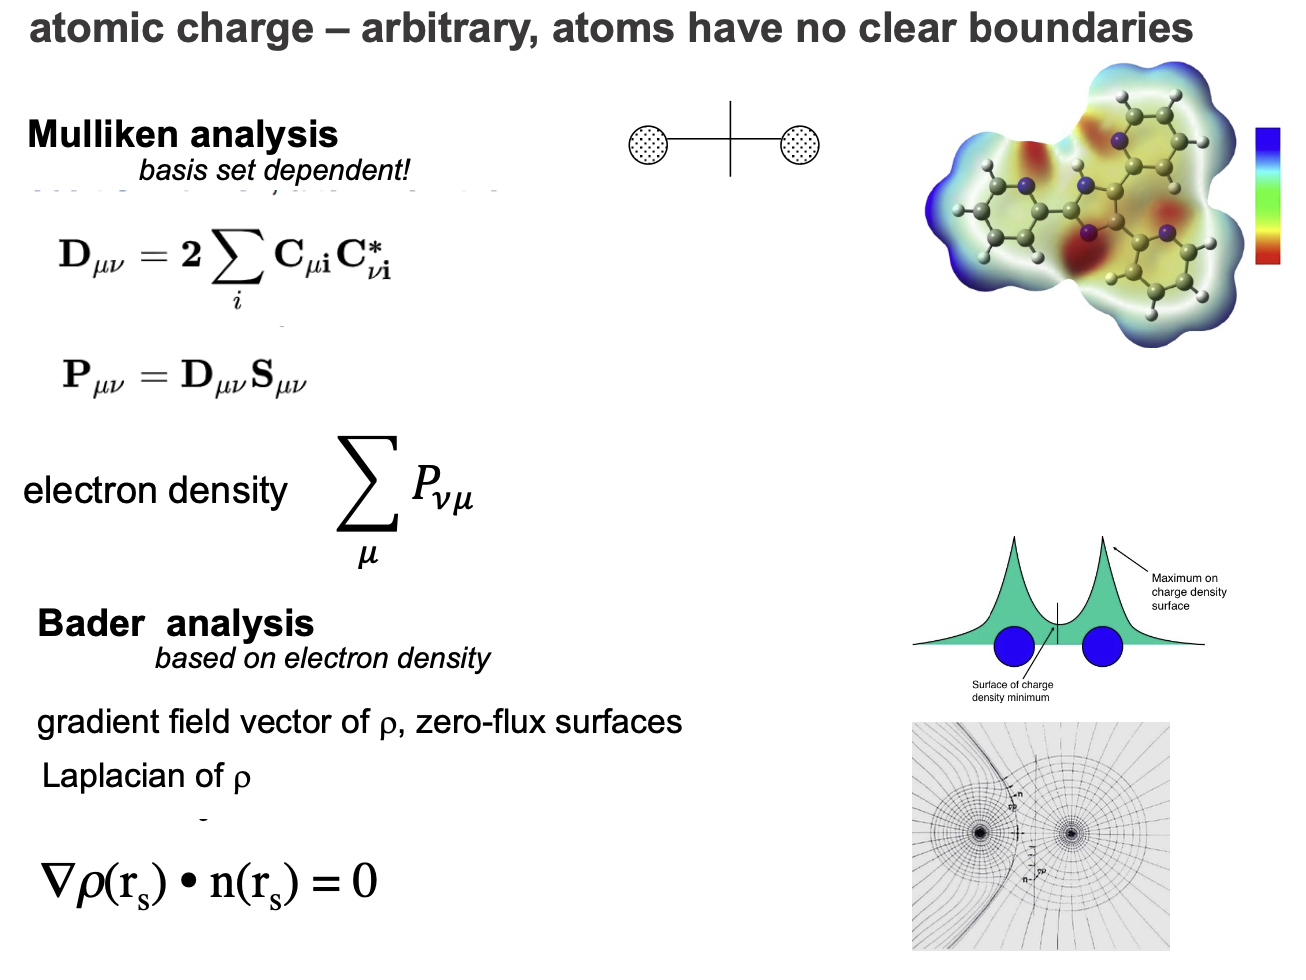
\includegraphics[width = 0.48\textwidth]{slides/simulations/atomcharge1.png}
    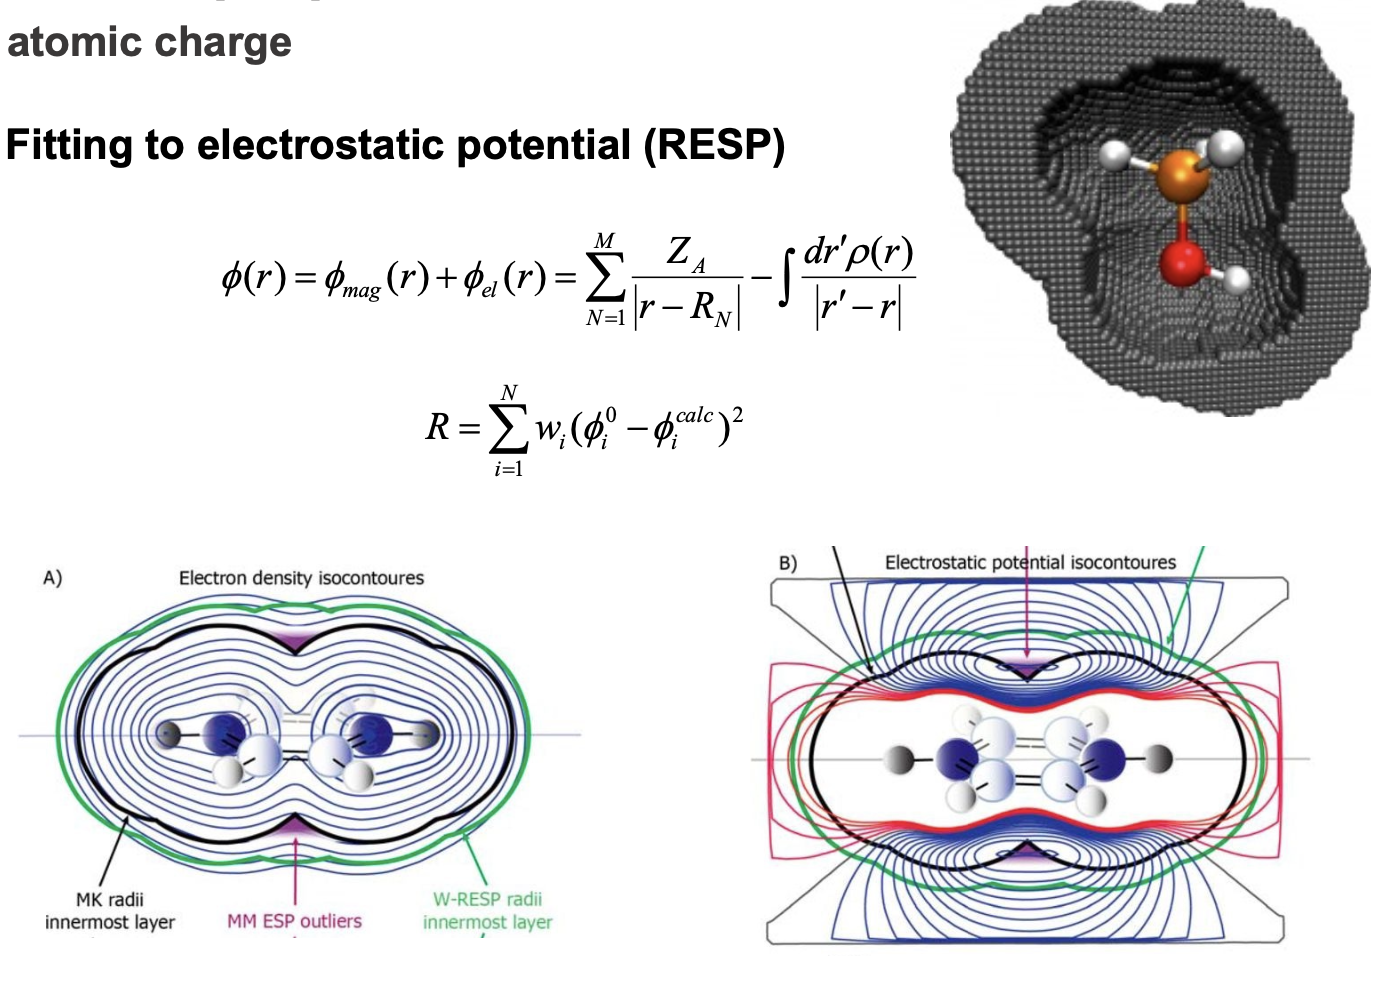
\includegraphics[width = 0.48\textwidth]{slides/simulations/atomcharge2.png}
    \caption{Methods for assigning atom charge}
\end{figure}


Now if you had some experience in molecular orbital calculations, you can do a so-called Mulliken population analysis. So basically you take the average of the coefficients. But this is would be like, you know, exactly halving the electrons which are shared on a molecular orbital. This is of course not a good approximation. 

Then you can be very sophisticated—this is the so-called Bader analysis, when you start analyzing basically the shapes of these molecular orbitals and you try to find the inflection points and you try to mathematically divide them. But I would say this is also pretty slow. 

\textbf{What works best and and used in most of the today's technology is a kind of simple but working method}. Okay? Many of many of the things in simulation are like this. So you try to make something effective that is that is not contrary to be correct. I think that's that's the expression for that. 

So basically what people do is as follows. \textbf{You can compute electrostatic potentials} from QM. And then basically you assign charges to the atoms and you try to \textbf{fit the potential}. What I'm assigning to the atoms is all artificial, it's non-physical. But what I'm getting at the end, it's physical. 






\subsection{Forces between atoms}

In a classical force field, the total potential energy is something like this:

$$
U = U_{bonds} + U_{angles} + U_{dihedrals} + U_{nonbonded}
$$

\begin{figure}[H]
    \centering
    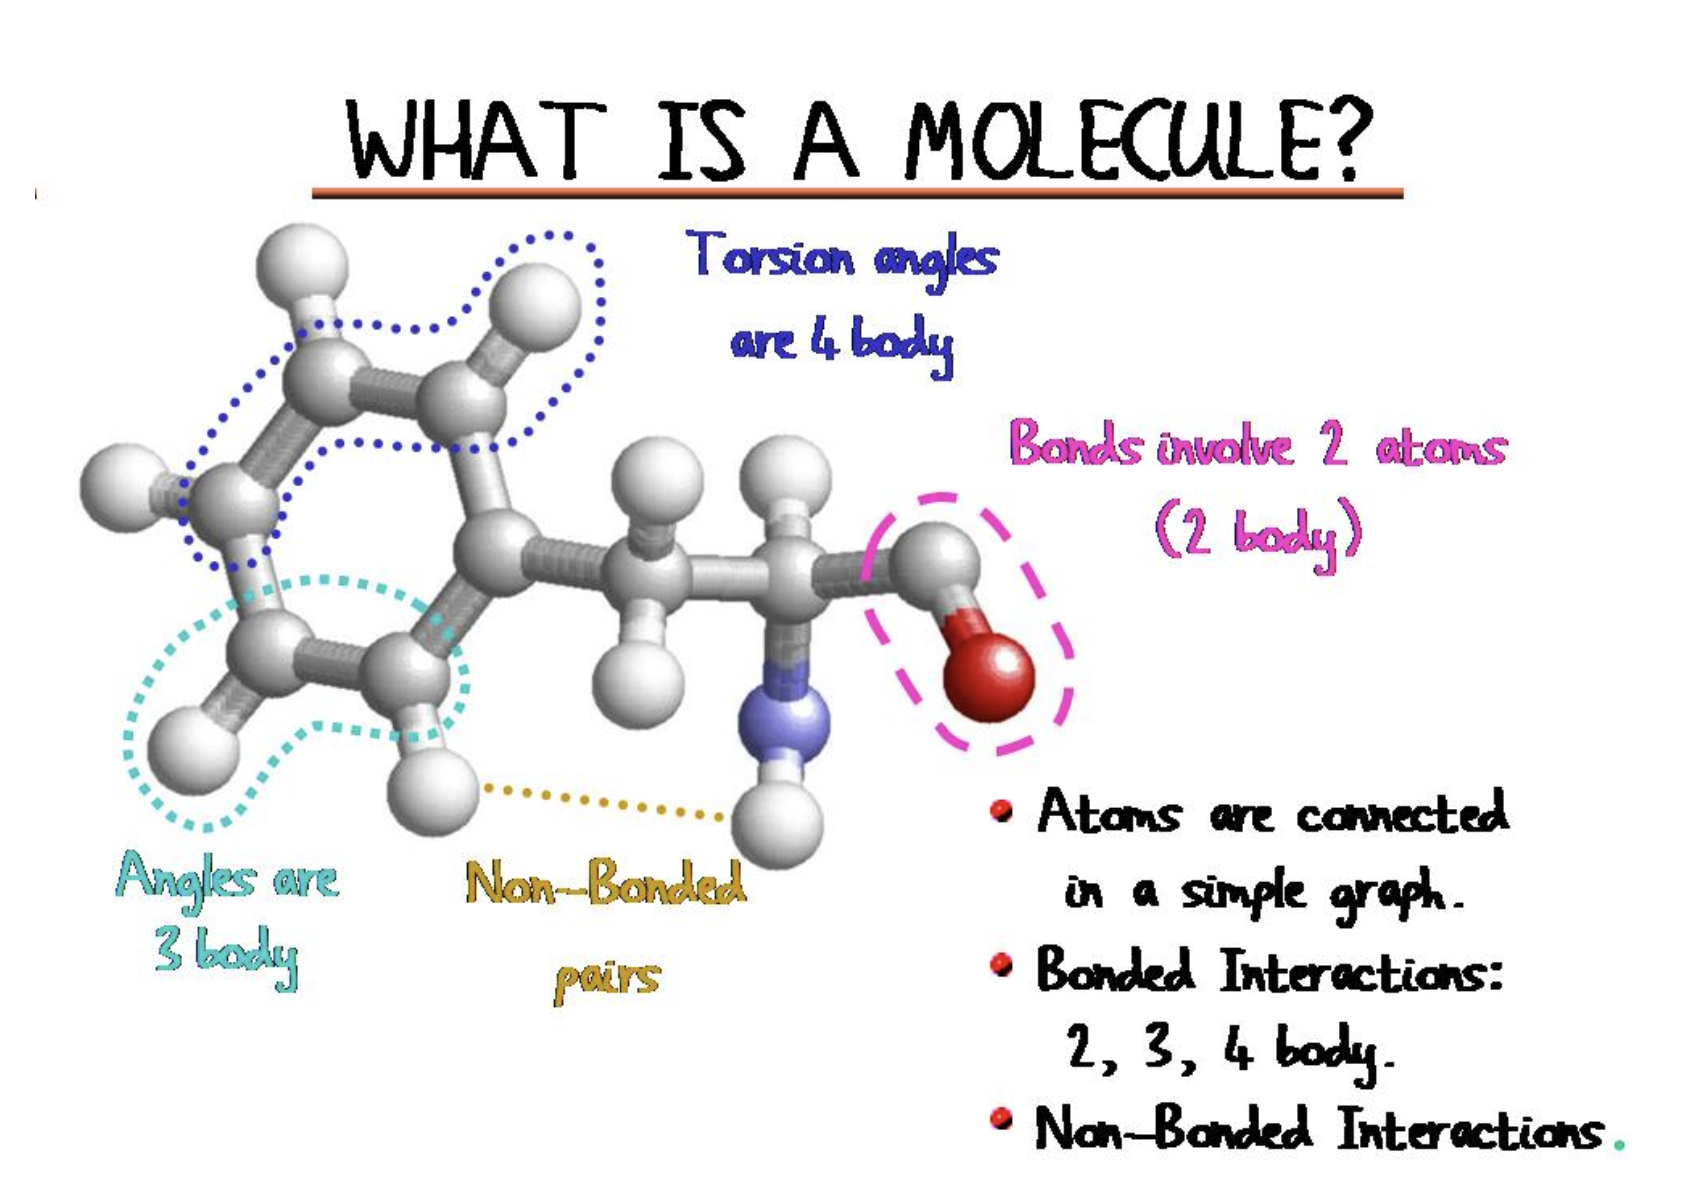
\includegraphics[width = \textwidth]{slides/simulations/234atoms.png}
\end{figure}


\paragraph{Bond stretch term}
So anyway, for bond stretching the k values are around in the order of hundreds, okay, quite large. Where do you get this, how do we know this?"
the bond length they are quite simple you get from x-ray crystallography. It's not that you need to generate they have been generated in the past century for small organic molecules, so basically they are all available. Okay. For the k you get them from infrared spectroscopy, which is kind of a vibrational spectroscopy. 
So when you put the Hook's law, you make this harmonic potential. So having said that, that means your bond will not break, cannot separate, I mean you won't vibrate to infinity. In case you want to break it, that would be almost quantum chemistry, then you need to apply some kind of different potential which is like for example a Morse potential, okay? Or you can take higher order terms, but this is almost never done because you can't pay for it in terms of the calculation.
\textbf{Remember this, that if you really want to break a bond for whatever reason in particular if you want to do quantum chemistry, you need either multi-scale or you just cannot apply molecular mechanics anymore.}

\paragraph{Bond angle term}
Next term, bond bending. So you try to describe a relationship between three atoms, okay? And also take some kind of harmonic term, some quadratic form."
and basically the rules are the same, you get these geometric terms from small molecule x-ray crystallography, which by the way has a resolution atomic resolution, okay? So it's below one Angstrom unlike proteins nowadays, okay? And you get the force constants from spectroscopy. \textbf{Here, the force constants kind of an order of magnitude smaller than those for the bond stretching}.

\paragraph{Torsion term}
You see here the approximate values, so they are very small, they are below $10 \, kcal/mol$, definitely. However, if you just do a simple combinatorial calculation, \textbf{you have so many of these 1 to 4 relationships that basically if you set this wrong, everything goes wrong. Because the bonds change very little, the angles change very little. However, these ones are the ones, if if you imagine this toy like a worm, these are the ones that actually move the protein}.
So this can basically mess up the whole calculation. 
Then there are these specific situations when you bind something to a ring or or something which is in a plane, then you have to define some specific terms to which is not a real torsion but but the deviation from the plane or deviation from you know some of the some of the ring atoms. This is rather technical. 

\paragraph{Modelling the hydrogen bond}
Okay. If I go on, the last issue in biomolecules, in particular proteins, is the hydrogen bond. and this had been a great question for quite long. I think I mentioned it one of my earlier lectures, I mean a hydrogen bond is typically shorter than a normal what you would expect from a normal Van der Waals relationship. and in the very very early force fields they treated hydrogen bond as separate."
But it's pretty difficult to treat, why? Because you don't see the hydrogens in proteins. You do see the hydrogens in small molecules but there you don't you see the hydrogen bond through crystalline packing but not through a real biological interaction. So this was I would say a nightmare to parameterize, also by ab initio it was a nightmare to parameterize. So anyway, to make the long story short, um it turned out that it is possible"
to describe the hydrogen bond as as kind of a summary of the Van der Waals interaction and the electrostatic interaction, which was I mean that was a critical point. From that moment biophysics could start that all the simulation of of biomolecules could start. Okay. The person who deserves the credit is Shneior Lifson, he did it in the early 70s. These are two students of of his, maybe I mention them later."


\subsection{How to choose the force field: some practical advice}

You don't need to develop a force field from the scratch, there will be parameters available. But \textbf{you have to make sure that all the parameters are defined}. Students usually like to rush it, and sometimes
the software doesn't tell you "look, you have this parameter absolutely missing" - sometimes they say but not always, and then they run two or three weeks and 'professor, I found one atom 2000 Angstroms away'. This usually happens because a force that should restrain that atom is missing, numerical integration keeps on going and the
atom files away.

In your lives you don't parameterize a force field from scratch for all the proteins. You borrow something that is adaptable to your type of protein.
But you may have a substituent, you may have a small molecule in particular a drug which is non-standard, which is not a biomolecule. So for those you may need to start from a quantum mechanical calculation, and you need translate it to the mechanical parameters that you need in your force field.

\paragraph{Empirical "ad hoc" adjustments are common. A FF typically only gets \textit{some} experimental observables right}
Now for the electrostatics interaction, um I mean you have the charges, the charges are you know you took somewhere you are aware of it. Um then you need to you need to manipulate the things. Either you introduce a dielectric constant which you didn't mean to introduce but but maybe some scaling. In a few cases you may introduce modifications when you have for example some evidence from quantum chemistry that there is polarization ongoing."
So here you often need to do fudging, I would say. Or what you can also do this is also a typical situation in a project that you put a molecule you want to neutralize, you put ions around it, and you put the ions too close. So your molecule doesn't move, 'professor, why the molecule doesn't move?'. You need to put the ions a bit away and then you know you compensate some of the polarization effects and that's it. Okay. So I mean you can"
The developers adjusted the FF for this property or that property. So you can choose some of these in particular structures pair correlation functions are often used, dipole moments are often used, density, and and you try to you try to optimize them. Don't believe that if you have a good force field you can validare all the properties [of the phys. sys]. Be happy if you can reproduce one or two.
So making a simulation is beautiful, we learned a lot from those, but still understand that they they suffer from major limitations. 


\paragraph{The most sophisticated model isn't necessarily the most effective}
\begin{figure}[H]
    \centering
    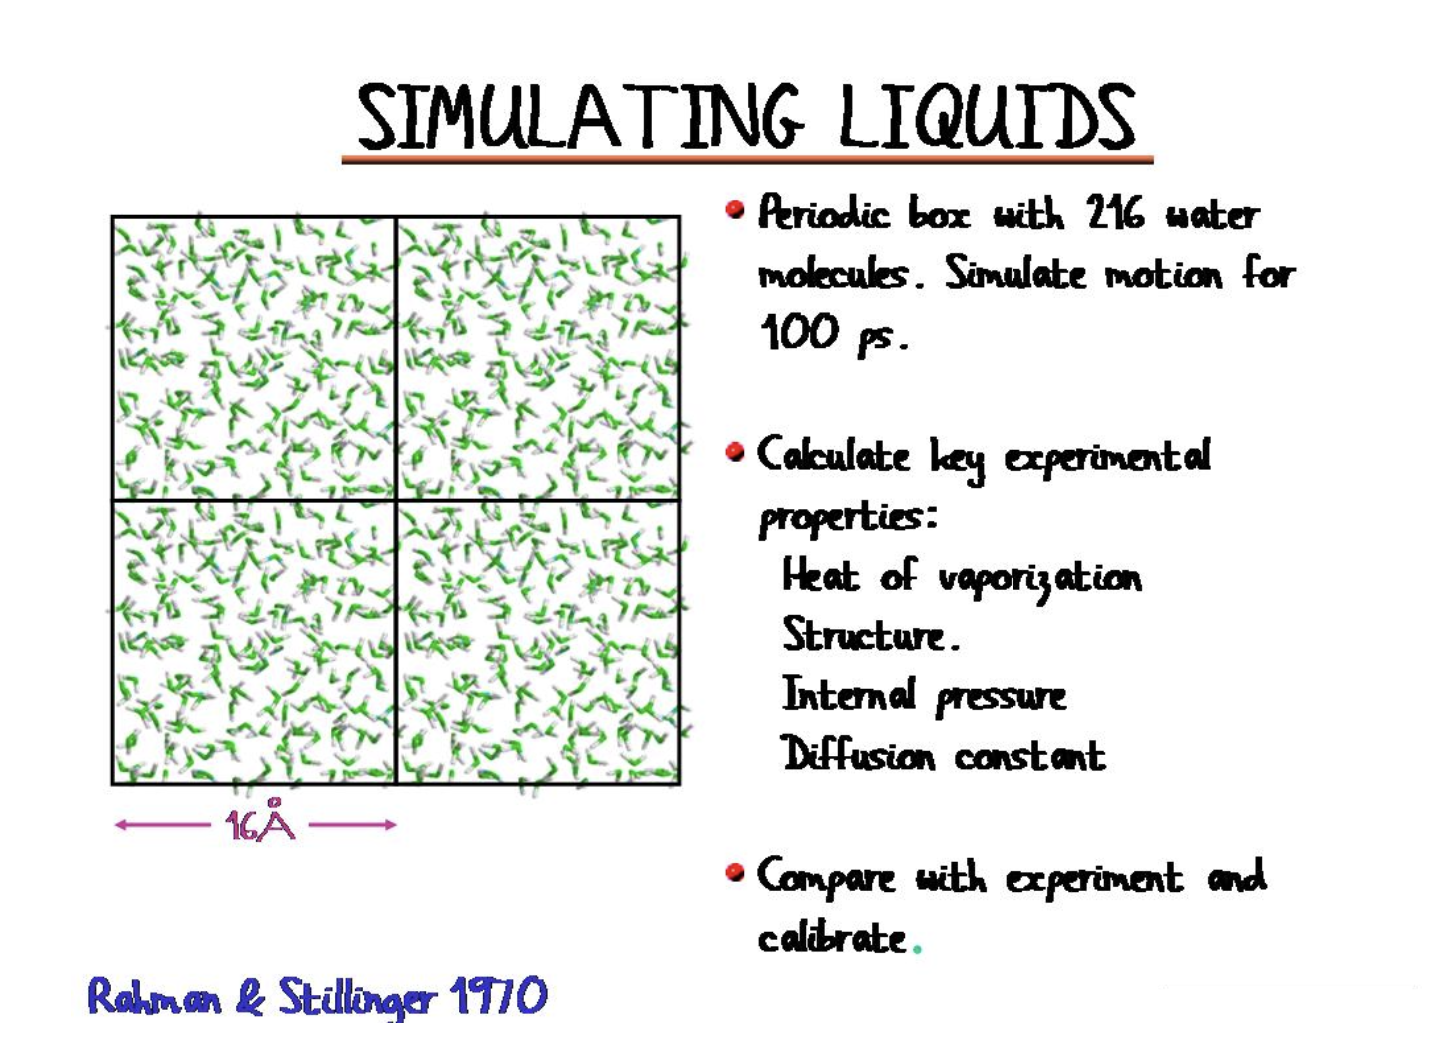
\includegraphics[width = 0.48\textwidth]{slides/simulations/liquid_sim.png}
    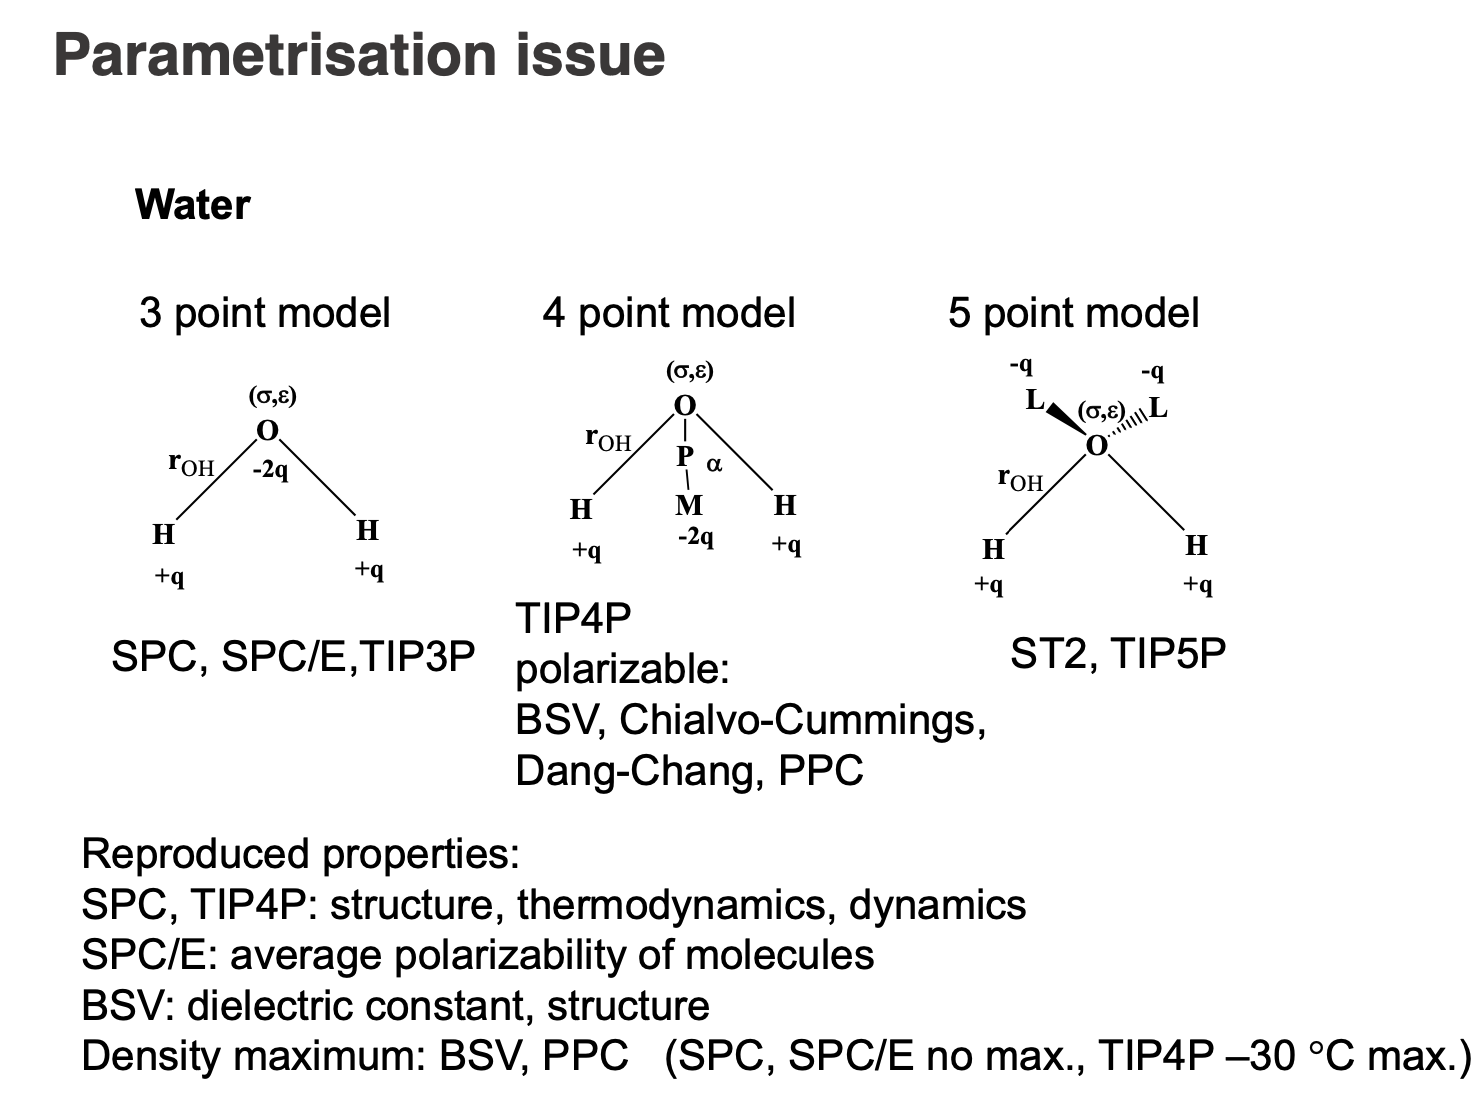
\includegraphics[width = 0.48\textwidth]{slides/simulations/liquid_res.png}
\end{figure}

Liquids are the simplest systems to simulate.
"You see how the models were developed, they didn't put here the year. So this is three point what water is like three atoms. Then four point one is specific for the for the non-bonded pair of the oxygen. Or you have five points where you have both of the non-bonded pairs represented specifically. There are different names, you can check in the literature. But look at this thing."
"I mean you may expect okay the five point is is the best because you know it's the most sophisticated. But no. Reproduce properties, structure, thermodynamics, dynamics, already you know three properties STD. One of the oldest reproduces all these three. Uh by the way if I look at it very carefully, TIP5P doesn't reproduce any, and then the density maximum is the PPC, which is four points."
"You can see TIP4P has a density maximum minus 30 and so on. So you can see this. So what you need to understand at this at this point, all this is very challenging, not impossible, there have been millions and millions of simulations done, maybe 60$\%$ of them were not correct because of banal errors even today, even in high impact journals, don't believe that it's not happening. 
But anyway, if you decide to use a simulation approach, you decide what is the property you are interested in, you have to ask the questions in an intelligent manner. You may parameterize also for solvation free energy or you know something that is relevant to your problem. And so you can do it, you just need to be aware if I'm parameterizing for solvation free energy then I'm not asking the question how the what is the rotation time of a certain group whatever."


\paragraph{Choosing an appropriate force field}

\begin{figure}[H]
    \centering
    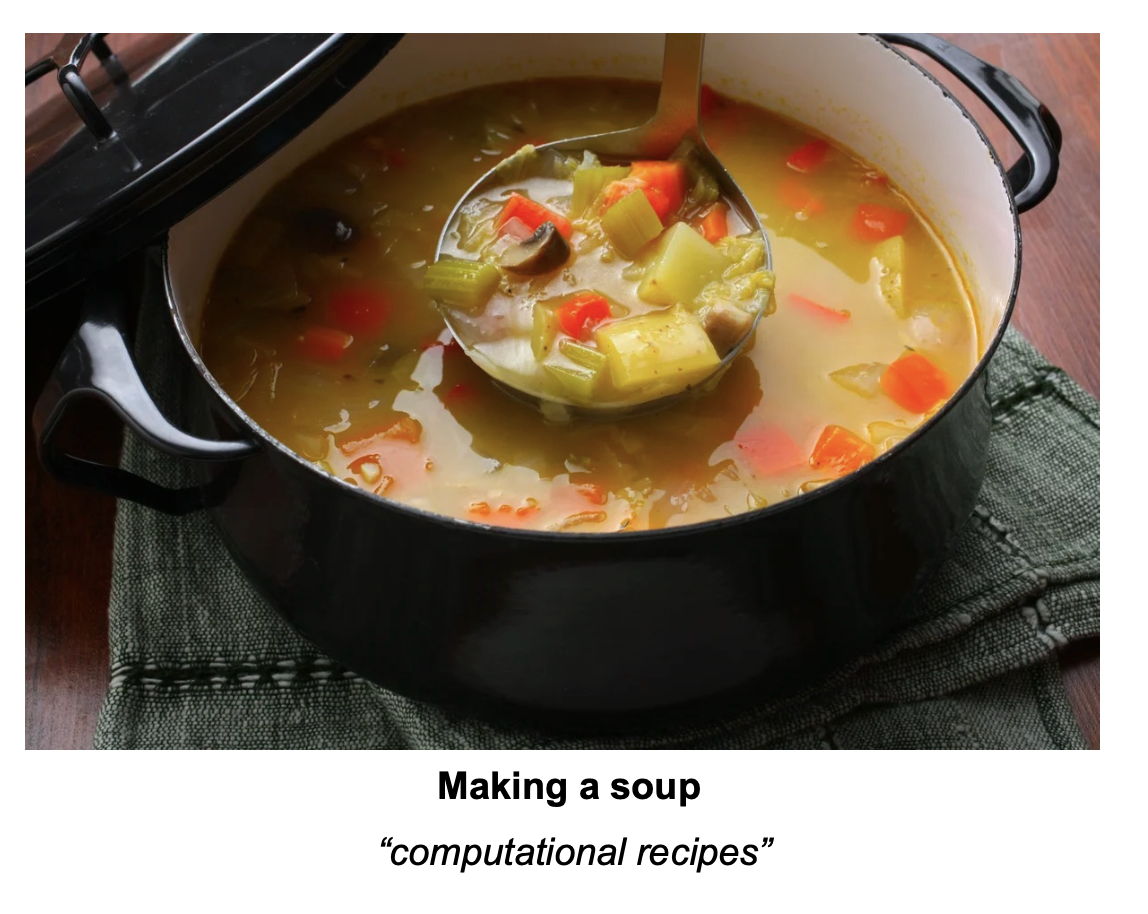
\includegraphics[width = 0.7\textwidth]{slides/simulations/soup.png}
\end{figure}


You need to be aware that you cannot make a better soup than the ingredients. So force fields are the heart at the core of all the simulations. Your simulation cannot be better than your your force field.
So you know if you have a force field developed for absolutely solid ordered proteins, you would never get a very dynamic system right, okay? 
So you must be aware of the limitations from the very beginning but even when you start making your soup even when you before you touch the very first button of the simulation you should have some ideas what you can get out of that simulation what you what you cannot get out of the simulation. 
In terms of time, in terms of spatial constraints or number of atoms, in terms of dynamicity and so on and so forth. 

You may even get unphysical results, very often it's happening. For example if there was a force field that was developed with ions, and then you forget to put ions into your simulations or vice versa, there can be a force field which was developed kind of in implicit environment and then you this is a DNA by the way and you start to put ions and you just see that it's
it's falling apart. So I mean you must be aware of the actual characteristics of the force field that you are using. Okay. 
These are some very classical force field, some of those do not exist anymore. some of those have always more modern versions normally numbered by year, for example the AMBER. It's called AMBER because there are always bugs in AMBER (!!).


\section{Multiscale MD}


\begin{figure}[H]
    \centering
    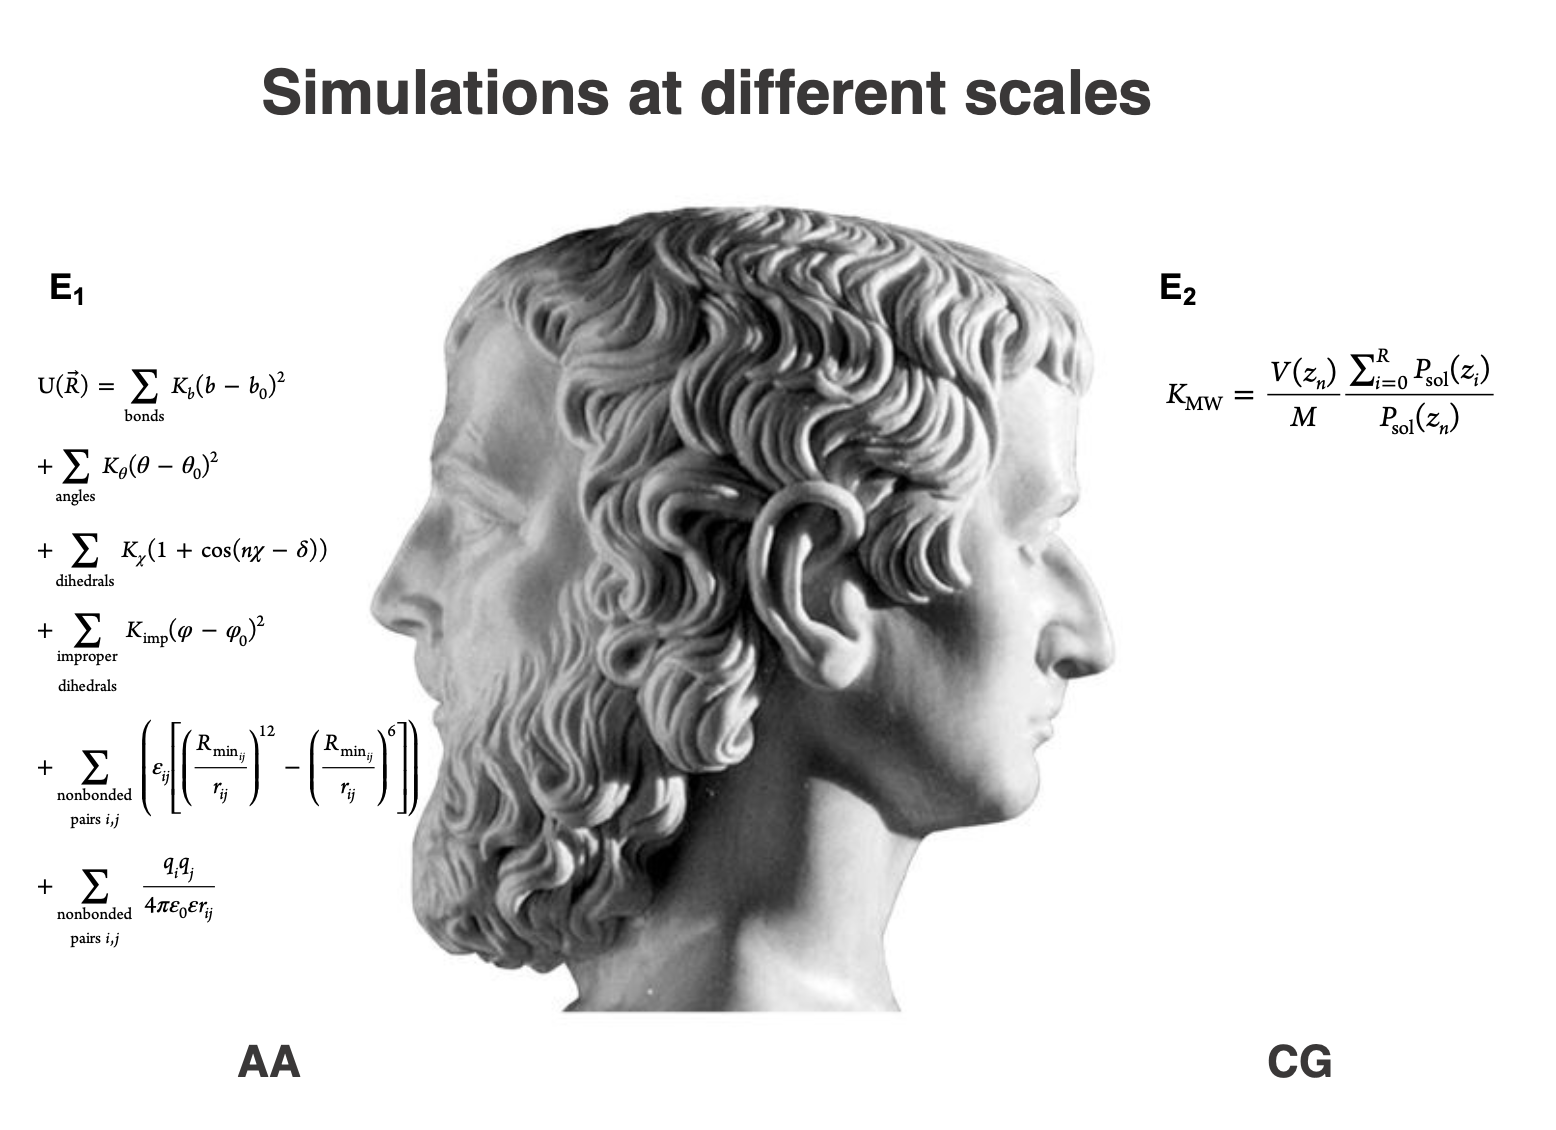
\includegraphics[width = \textwidth]{slides/simulations/giano.png}
\end{figure}

"if you let's say run into a problem which is fairly complex and you realize you can't do it at your scale. Now, this is a Janus space, Janus is a guardian of the of the ports in the Greek mythology. and uh so that's a problem. you can use for example this is an all atom potential again a generic one that we just discussed. This is for example a coarse graining potential. So if you"


"what if you you just don't find the right scale? So then you have to apply so-called multi-scale uh and in principle you know you can treat part of the system in one way and another part of the system in another way, but you may see or better not see the the cave out or the difficulty the challenge of this approach. Where I finish this and where this starts. So this could be another"


"or QM/MM these are the main approaches all atom coarse grain or QM/MM. So this is basically combining scales. and uh so the idea is that you need to generate it in a consistent manner that the forces wherever you put the interface the forces should balance. Because if you so that's kind of the limitation for for these technologies. It's not a problem that one"


"let's say one region is treated differently than another. The only point is when they meet the forces must be balanced. because if not this is from the early days, you can pull out let's say typical water molecules from one system to another, simply because the forces are larger towards another direction. So um this is kind of a an artifact. So um then the question is where the boundary is,"


"and what how do you compute the the forces at the boundary? and this is a field on its this is a field on its own, so I won't tell all the stories if you're kind of interested in you can see some graphs here that I I drew lots of things how you can take boundaries and I showed afterwards let's say what is the error in the force and you can see that in different situations you can have extreme differences"


"between the different systems. However, there are some solutions to this. don't even bother with the actual values just the fact that you can define these boundaries in very different ways and you can see that the errors differ markedly. So anyway the idea was implemented that you can take a zone here which is so-called the buffer zone, where you take the errors from both of the systems"

"and then you try to balance them. which looks simple but actually it's quite quite difficult. I show you I show you a particular application which is not biological although I could have shown also biological one. This is a crack propagation in particular in the in the wing of airplanes. So these technologies were really propelled about 20 years ago basically by the industry there were lots of accidents."


"and they didn't understand how the crack propagates. and there was a paper in Nature just dealing with this problem. Just dealing with how to define in a this you cannot do by MM, this you cannot do by QM because then the crack won't propagate because you can't simulate, so you have to deal with the multi-scaling QM/MM. But because it's moving the crack is moving you have to compute the errors and the error"


"estimates kind of being cold on the fly. So but that's the same thing if you were simulating let's say a protein channel an ion passing through a protein tube, okay in a membrane. that's the same kind of problem. But fortunately, fortunately not fortunately because of the accidents but fortunately because of the industry these technologies were sponsored. so there were a quite a few algorithms developed"


"to basically how to make this matching between the different um between the different scales. Again okay these are the three main issues. this picture which I'm always showing from one of my students, this was generated by a QM/MM. The first multi-scaling was actually published 1972, okay? and these are all the students of Shneior Lifson who got Nobel prize in 2013 Nobel prize in chemistry,"


"and it was claimed to be given for this hybrid approach QM/MM classical which is the MM the quantum and the combined term. But basically these three people founded computational biophysics overall. Okay. I put much more information always into the slides simply because if you want to have a look or you're interested in particular details you can have a look. but basically what I wanted to"


"just to kind of add with this little part that for you to understand that you learn to construct the potential energy surface in a certain manner, okay which was for all atom. that potential energy surface you can use to simulate conformational dynamics of proteins. but there are limitations, limitations of many kinds. If you don't use polarizable force field you won't see those effects those fine-tuned effects for example between aromatic groups and positively charged groups and so on."


"That may be critical for some kind of organization of proteins. You may not see chemical reactions simply because you take the bonds as harmonic so you cannot break them, okay? and also you can you will not be unlikely to see large changes simply because you cannot simulate enough. So you can modify these potential energy surfaces in a manner that you will be more efficient, let's say you can coarse grain,"

"but then the questions you ask may be different. Or you can also go to the other direction you can be more detailed about them. Maybe combining with all atom, but then new questions or new problems basically arise coming from the boundaries and the errors and the error compensation along the boundaries. So this is more or less what I wanted to share with you today about the force fields."
